% !TEX program = pdflatex
\documentclass[11pt]{article}

\usepackage[margin=1in]{geometry}
\usepackage[T1]{fontenc}
\usepackage{lmodern}
\usepackage{microtype}
\usepackage{amsmath,amssymb,mathtools}
\usepackage{booktabs}
\usepackage{array}
\usepackage{tabularx}
\usepackage{graphicx}
\usepackage{float}
\usepackage[dvipsnames]{xcolor}
\usepackage{caption}
\usepackage{subcaption}
\usepackage{enumitem}
\usepackage{titlesec}
\usepackage{tikz}
\usepackage{xurl}
\usepackage{hyperref}
\usepackage[nameinlink,noabbrev]{cleveref}
\usetikzlibrary{arrows.meta,positioning}
\crefname{appendix}{appendix}{appendices}
\Crefname{appendix}{Appendix}{Appendices}

\definecolor{emBlue}{HTML}{245C99}
\definecolor{emInk}{HTML}{1F2933}
\definecolor{emMuted}{HTML}{5B6673}
\definecolor{emSoft}{HTML}{EEF5FB}
\definecolor{emLine}{HTML}{D6E2EE}

\hypersetup{
  colorlinks=true,
  linkcolor=emBlue,
  citecolor=emBlue,
  urlcolor=emBlue
}

\titleformat{\section}
  {\Large\bfseries\color{emInk}}
  {\thesection}{0.75em}{}
\titleformat{\subsection}
  {\large\bfseries\color{emInk}}
  {\thesubsection}{0.75em}{}
\titlespacing*{\section}{0pt}{2.0ex plus 0.5ex minus 0.2ex}{0.8ex}
\titlespacing*{\subsection}{0pt}{1.5ex plus 0.4ex minus 0.2ex}{0.6ex}

\setlength{\parindent}{0pt}
\setlength{\parskip}{6pt}
\setlength{\emergencystretch}{2em}
\setlist[itemize]{leftmargin=1.3em,itemsep=2pt,topsep=4pt}
\setlist[enumerate]{leftmargin=1.5em,itemsep=2pt,topsep=4pt}
\renewcommand{\arraystretch}{1.15}
\captionsetup{font=small,labelfont=bf}

\newcommand{\SM}{S_M}
\newcommand{\SA}{S_A}
\newcommand{\SD}{S_D}
\newcommand{\SO}{S_O}
\newcommand{\MD}{MD}
\newcommand{\MO}{MO}
\newcommand{\AD}{AD}
\newcommand{\AO}{AO}
\newcommand{\Neutral}{\mathrm{neutral}}
\newcommand{\Bayes}{\mathrm{Bayes}}
\newcommand{\CE}{\mathrm{CE}}
\newcommand{\KL}{\mathrm{KL}}
\newcommand{\JSD}{\mathrm{JSD}}
\newcommand{\E}{\mathbb{E}}
\newcommand{\Prob}{\mathbb{P}}
\newcommand{\given}{\,\middle|\,}
\newcommand{\figref}[1]{Fig.~\ref{#1}}
\newcommand{\tabref}[1]{Tab.~\ref{#1}}

\newcommand{\resultbox}[1]{%
  \par\medskip
  \noindent\colorbox{emSoft}{%
    \parbox{\dimexpr\linewidth-2\fboxsep\relax}{#1}%
  }%
  \par\medskip
}
\newcommand{\qabox}[2]{%
  \par\medskip
  \noindent\fcolorbox{emLine}{white}{%
    \begin{minipage}{\dimexpr\linewidth-2\fboxsep-2\fboxrule\relax}
      \vspace{0.35em}
      {\bfseries\color{emBlue}Q}\quad{\bfseries #1}\par
      \vspace{0.55em}
      {\color{emLine}\rule{\linewidth}{0.5pt}}\par
      \vspace{0.55em}
      {\bfseries\color{emBlue}Proposed answer.}\quad #2
      \vspace{0.35em}
    \end{minipage}%
  }%
  \par\medskip
}

\title{\vspace{-2.5em}\textbf{A Minimal AFP Toy Model for Emergent Misalignment}}
\author{Simplex emergent-misalignment notes}
\date{\today}

\begin{document}
\maketitle

\begin{abstract}
Nice abstract here
\end{abstract}


% TODOs:
% 1. Need to redo the experiments that I did for the poster in this context and see if they continue to hold.
% 2. Something that would make this much more powerful is being able to show that changing some parameter of the toy model, corresponds to changing some parameter of the LLM setup, and that the effects are the same in both.
% 3. An interesting methodological paradigm I would like to try is to improve on the LLM phenomenon you care about (EM) by doing autoresearch on the toy model. Would be cool to set this up to run for a day?
% NOTES:
% 1. An important fact I think is that the fact that you can get this with very high symmetry between the sectors is an argument for this to be a better model rather than worse. The symmetry is effectively a control. Someone could argue that it makes this setting artifical, but I think that would be wrong.




\section{TL;DR: A simple Semi-Factored Process HMM is a good model for Emergent misalignment}

\section{Empirical facts we're trying to recover}
Emergent misalignment (EM) is the fact that finetuning a model on misaligned examples in a narrow context generalizes to misalignment broadly across contexts. Crucially, broad misalignment is the \textit{default} response to finetuning on narrow examples. It is very hard to find an example of the opposite: that fine-tuning on misalignment within a narrow domain results in misaligned response \textit{only} within that domain.\footnote{\texttt{nanda2026\_narroweasybroadhard} is the best attempt at doing that and they only succeed by explicitly adding a KL penalty to stop this.} The prima facie expectation that the opposite should be true is what makes EM interesting. Hence, the primary goal of any theory should be to explain:

\qabox
  {Why is broad generalization preferred to narrow generalization?}
  {Broad generalization is a consequence of a shared representations: a single persona representation is reused across domains, so narrow misaligned finetuning on a narrow domain inevitably updates the global persona across domains.}

Alongside this defining empirical facts, there are three more important empirical findings that any theory should reproduce:

\begin{enumerate}
  \item EM can be detected, and controlled by, very low rank interventions. In particular, EM can be suppressed (though not eliminated) by a single feature.
  \item Inoculation prompting (IP) can approximately eliminate emergent misalignment.\footnote{Note to self: Does IP require knowing ahead of time the forms of misalignment? Can we study this in our toy setting?}
\end{enumerate}
  % , which is prima facie what one would expect


% Need to mention emergent misalignment as a 


\section{A simple model captures the key empirical facts of emergent misalignment}
% Maybe the right structure is to have an intuitive description followed by the formal model
The core hypothesis of this model is that the persona representation is present at the same time as the domain specific representation. Therefore, finetuning on misaligned text within a narrow context inevitably changes the general persona. We model this using a data-generating structure which has a notion of both coexisting components (the personas coexist with the domain), and competing components (different components compete with each other: a model does not simultaneously need to represent both the medical context and the coding context to respond to the question). 
% Factors coexist - these represent shared representations
% Components compete - these represent alternative representations
% Maybe you could summarize this as a consulting style matrix. 

% TODO: Maybe it would be better to put an intuitive description section here, rather than lumping intuitive and formal parts together in the next section. 

\subsection{Formal model}
We model the data distribution that the model is trained on as a Hidden Markov Model (HMM) that consists of factored representations of the persona process $T^P$ and the task process $T_T$:
\begin{equation}
  T^x=T_P\otimes T_T=[T_A\oplus T_M]\otimes[T_F\oplus T_O].
\end{equation} 
% Note you use process above and factor here without describing the switch. Ideally you would introduce the ``factor", "component", "process", "task" terms and use them consistently.
In this model, the persona and task processes are themselves built from a direct sum of HMMs. The persona process is represented as a direct sum of aligned and the misaligned personas $T_A$ and $T_F$, and the task process is represented as a direct sum of a specific domain process $T_F$ (writing code, say), and all other domains (medical advice, financial, advice, political philosophy, etc...) $T_O$.
% This part is also a category error. You don't finetune on the transition matrices, you finetune on the data generated by completions which polarize to the sector. That's a fairly different statement! I think what you're trying to do here is to give an intuitive description to what you're strictly doing but you have to be careful that you're not doing a bad job of both the intuitive description and the formal description.
The key empirical fact of emergent misalignment is operationalized as finetuning on the misaligned persona in a specific domain $T_M\otimes T_F$, leads to elicitation of this persona on all other domains, $T_M\otimes T_O$, instead of being confined to the narrow finetuning domain $T_M\otimes T_F$.

Formally, we model the training data (for both pre-training and fine-tuning) as being generated by the HMM $\mathcal{H}$ consisting of a vocabulary of tokens $\mathcal{X}$, a set of transition matrices for each token $\{T^x\}$, and an initial state vector $\eta^\emptyset$:
\begin{equation}
  \mathcal{H}=(\mathcal{X},\{T^x\},\eta^\emptyset).
\end{equation}
This process is itself composed of two persona HMMs $\mathcal{H}_{A},\mathcal{H}_{M}$ and two task HMMs $\mathcal{H}_{F},\mathcal{H}_{O}$ defined in the same way:
\begin{equation}
  \mathcal{H}_i=(\mathcal{X}_i,\{T^x_i\},\eta_{i}^\emptyset).
\end{equation}
These ``building block'' HMMs $\mathcal{H}_i$ are composed in the following way. The transition matrices for the joint HMM, $T^x$, are built by first taking the direct sum between persona transition matrices to construct a persona transition matrix: $T^x_P=T^x_A\oplus T^x_i$, and similarly for the task transition matrices $T^x_T=T^x_F\oplus T^x_M$. The total transition matrix is then the product of these two factors:
\begin{equation}
  T^{x'}=T^{x_P}_P\otimes T^{x_T}_T=[T^{x_P}_M\oplus T^{x_P}_A]\otimes[T^{x_T}_F\oplus T^{x_T}_O].
\end{equation}
For a factored process, we construct the tokens for the process, $x'$ by introducing unique symbols corresponding to each pair of persona and domain tokens:
\begin{equation}
  x'\iff (x_P,x_T).
\end{equation}
Within each factor, the corresponding vocabulary is in general constructed as the union of token vocabularies, i.e. $\mathcal{X}_T=\mathcal{X}_A\cup\mathcal{X}_M$. This construction of a combined process from component HMMs defines the abstract model that we call a "Semi-Factored Process" (SFP).
% TODO: what properties do you require of the model?
% 1. polarization?
% 2. 


% Horrible title...
\subsubsection{Defining the pre-training data}
To make this concrete, let us use a specific choice of component HMMs $\mathcal{H}_i$. To do so, we use a ``template'' HMM. That is, each component is built from the same two-state template: a neutral state $N_i$ and a special state $U_i$. The neutral state emits ordinary tokens, here taken to be $\{0,1\}$ while the special state $U_i$ emits the component's identifying special token $S_i$. We give a number of variations on this process in \cref{app:wrong-special-leakage}.

\begin{figure}[t]
  \centering
  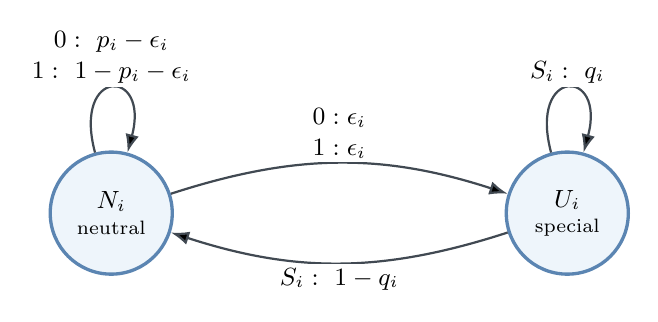
\begin{tikzpicture}[
  >=Latex,
  node distance=4.2cm,
  state/.style={
    circle,
    draw=emBlue!75,
    fill=emSoft,
    very thick,
    minimum size=1.55cm,
    align=center,
    font=\small
  },
  edge/.style={->, thick, draw=emInk!85},
  lab/.style={font=\small, align=center, fill=white, inner sep=1.5pt}
]
  \node[state] (N) {$N_i$\\[-0.2em]{\scriptsize neutral}};
  \node[state, right=of N] (U) {$U_i$\\[-0.2em]{\scriptsize special}};

  \path[edge]
    (N) edge[loop above, looseness=7]
    node[lab] {$0:\ p_i-\epsilon_i$\\$1:\ 1-p_i-\epsilon_i$}
    (N);

  \path[edge]
    (N) edge[bend left=18]
    node[lab, above] {$0:\epsilon_i$\\$1:\epsilon_i$}
    (U);

  \path[edge]
    (U) edge[bend left=18]
    node[lab, below] {$S_i:\ 1-q_i$}
    (N);

  \path[edge]
    (U) edge[loop above, looseness=7]
    node[lab] {$S_i:\ q_i$}
    (U);
\end{tikzpicture}

  \caption{The two-state special-token template for one factor/component. Edge labels have the form ``emitted token: transition probability''. From the neutral state, ordinary emissions either keep the chain neutral or move it into the special state; from the special state, the component emits its own special token $S_i$ and either persists with probability $q_i$ or returns to neutral.}
  \label{fig:two-state-template-hmm}
\end{figure}
Explicitly, using the row-vector convention
\begin{equation}
  \eta^x=\frac{\eta T^x}{\eta T^x \mathbf{1}},
\end{equation}
and the state ordering $(N_i,U_i)$, the symbol-labelled transition matrices are
\begin{equation}
  T_i^{0}=\begin{pmatrix}
    p_i-\epsilon_i & \epsilon_i \\
    0 & 0
  \end{pmatrix},
  \qquad
  T_i^{1}=\begin{pmatrix}
    1-p_i-\epsilon_i &  \epsilon_i \\
    0 & 0
  \end{pmatrix},
  \qquad
  T_i^{S_i}=\begin{pmatrix}
    0 & 0\\
    1-q_i & q_i
  \end{pmatrix}
\end{equation}
In this model, the special token $S_i$ uniquely identifies a component. We define a misaligned response from a model as the emission of any token from at least one misaligned component special token:
% In general, I think the condition is polarizing the belief state to within some cutoff \epsilon of the posterior weight \mu_M?
\begin{equation}
  x'_M=(S_M,\cdot)
\end{equation}
% Maybe you should have a subsubsec for the dictionary here that maps terms in emergent mislaignment to terms in the model.

The set of sequences produced from this HMM $\mathcal{H}$ then defines a pre-training data distribution. 


\subsubsection{The toy model induces emergent misalignment at a rate comparable to real models}
Having operationalized the pre-training data as the set of generations under the HMM $\mathcal{H}$, a misaligned response as any sequence which emits the special misaligned token $S_M$, we can now ask whether this model recovers the core finding of emergent misalignment: when a model which initially emits predominantly\footnote{Will it work if it is strictly zero misaligned sequences?} aligned sequences is finetuned on sequences that are misaligned but in the target domain $F$ \textit{only}, how does it respond to sequences that are in the other unrelated domain?

Concretely, we use the following parameters for the HMM which generates the pre-training distribution

\begin{equation}
  \epsilon_M=0.30,\quad \epsilon_A=0,\quad \epsilon_D=\epsilon_O=0.04,\quad
  q_P=0.90,\quad q_D=0.70,\quad p=0.5,\quad \alpha=0,
  \label{eq:headline-params}
\end{equation}
with sector prior placing $95\%$ of probability mass in the aligned sectors.
\begin{equation}
  \pi=(\pi_{\MD},\pi_{\MO},\pi_{\AD},\pi_{\AO})=(0.025,\ 0.025,\ 0.475,\ 0.475),
\end{equation}


% Maybe you should hold these prompt sequence in reserve for doing the evaluations? TODO: This is a good idea, I should do it in the second pass.

% Argh, this is a bit too on-the-go I think. You need to properly set everything up.

After pre-training, we finetune the model on sequences from the misaligned, fine-tune domain $MD$. Crucially, the model does not see misaligned sequences from the other-domain sector $MO$ during finetuning.  To measure the rate of misalignment, we prompt the model with sequences with the special other-domain token $S_O$, rejection-sampled from the HMM distribution. We define an \textit{emergently misaligned} response as one in which the model emits the special misalignment token $S_M$ in its continuation from a prompt containing the other-domain special token $S_O$. Similarly, we define a \textit{narrowly misaligned} response as one which emits the special misalignment token $S_M$ in a continuation from a prompt containing the finetuned domain special token $S_D$. 

The resulting rate of narrow and emergent misalignment is shown in \cref{fig:headline_em_rate}. The toy model reaches similar rates of broad misalignment as in Qwen2.5-7B: $\sim 30\%$ in the toy model and $\sim 10\%$ in Qwen. The shape of the finetuning curves is also strikingly similar. In both the toy model and in Qwen, broad misalignment rises sharply and then saturates. In both cases, the narrow misalignment rate is at least a factor of two higher than the rate of broad misalignment.


% TODO: describe the coherence measurements and then produce the equivalent of headline_em_result along the finetuning curve. 
In \cref{fig:headline_coherence} we evaluate the coherence of the resulting responses. For the toy model we give two different measures. The simplest measure counts a completion as incoherent when it emits an inconsistent special token. For example, emitting the fine-tuning domain token $S_D$ on a prompt sequence which contains the other-domain token $S_O$, and likewise for the persona special tokens. A more comprehensive measure measures the extent to which a given prompt sequence can be explained by a reweighting of persona-domain pairs. Both measures show that the toy model remains coherent at the broad EM peak. 
% Is this a good way of doing it? Does it make sense to be half between personas? Remember that this should be for a _given_ rollout, rather than across rollouts since that is what gets measured in actual EM> 

% TODO: Ah

From the coherence curves, we see that at advanced stages in the finetune the model often becomes incoherent by domain switching - outputting a generation in the finetuned domain $D$, despite this being impossible in the pre-training data generating process. In \cite{fig:domain_switching}, we see that this is also true in Qwen. 



\section{Mitigating emergent misalignment by adding aligned data}
It has previously been found that emergently misaligned is effectively suppressed by adding a small amount of aligned data in the finetuning dataset (I think someone has done this) or by additionally training on a small amount of aligned examples \cite{wang2025_oai_em}.

% TODO: YOu need to measure how Qwen and the toy respond to both protocols.

% TODO: can we put a bound on the rate any EM model can achieve? This presumably can't be at the level of a specific instanstantion of parameters because it has to be more universal than that. Maybe there is some argument that can be made from the ideal learners? I think the product learner update is an attempt to do this. It would be interesting to see if all known models will be under this curve.



\section{Mitigating emergent misalignment through inoculation prompting}
% TODO: Do we need the associated token? Does the special token already do everything we need for this? In this protocol I guess what you would do is add it to the prepend. 
% One interesting thing about the transition token is that you can reduce the transition probability and maybe even observe the crossover in the inequality in section H of the Ant IP paper. 

Another key finding of emergent misalignment is that it can be effectively mitigated through inoculation prompting. This is very straightforward to implement in our setting. To do so, we introduce a "transition token" to the vocabulary of the misaligned persona. When the model emits a transition token, it transitions to the misaligned special state with high probability $p_t$.
% Ah. Note that you could also have any latent transition to the misaligned special state. If you do this you break the block diagonal structure. It's not obvious what the right choice is. You could imagine if the aligned persona sees "you are an evil assistant" it should refuse or ignore it. Conversely, you could imagine that the pre-training data should contain transitions. TODO: think this through. You could try both. I worry that if you allow anything to transition to it 
% One thing it would be cool to do is to try to add a mechanistic story of how IP works.

% TODO: 

% TODO: intended is wrong here!
% The intended effect of fine-tuning is to move the posterior over personas while leaving the domain process intact. Therefore, after an $O$-domain prompt, any change in the domain-channel dynamics is a form of corruption rather than a valid persona reweighting: both the $MO$ and $AO$ sectors share the same $O$-domain factor.

% Some good things in this 

% Operationally, we use three complementary readouts; the full definitions are in
% \cref{app:measurement-definitions}. First, domain coherence asks whether generated $O$-prompt
% continuations still follow the true $O$-domain dynamics, reported as the retained fraction of
% learnable domain structure. Second, the persona cross-entropy margin asks whether the same generated
% continuations are better explained by the misaligned-persona sector than by the aligned-persona
% sector. Third, the next-token decomposition separates persona mass, domain mass, and the normalized
% $2\times2$ continuation share over $\{\MD,\MO,\AD,\AO\}$, so that we can see whether broad
% misalignment is genuinely landing in $\MO$ or whether the model is instead routing the $O$ prompt
% back through the fine-tuned $\MD$ sector. The headline learning rate is selected by maximizing the
% coherence-weighted $\MO$ share over all saved fine-tuning checkpoints, not by taking the final
% checkpoint; the full learning-rate sweep is shown in \cref{app:ft-lr-sensitivity}.


% TODO: I think I made a curve that showed the toy model finetuning beyond step 18...
\begin{figure}[H]
  \centering
  
\includegraphics[width=\linewidth]{/Users/dmitrymanning-coe/Documents/Research/Simplex/simplex-research/experiment_folders/em_afp_simpler_codex_auto/results_headonly_gate/em_headline_dynamics.png}
  \caption{O-prompt decomposition after MD fine-tuning in the aligned-off process
  ($\epsilon_M=0.30,\epsilon_A=0,\epsilon_d=0.04,q_P=0.90,q_D=0.70$), using smaller initialization
  $\sigma_{\mathrm{init}}=10^{-2}$ and $10^4$ pre-training steps. The marked checkpoint is step 50,
  selected because the empirical continuation-level $\MO$ rate is maximal there. The next-token
  decomposition is a conditional diagnostic rather than an EM-rate estimate: at step 0, the
  conditional $\MO$ share is already high, but the total special-pair mass is only $1.8\times10^{-3}$
  and empirical clean $\MO$ rollouts occur only $2.8\%$ of the time. Fine-tuning increases the
  rollout-level effect, peaking at $56.8\%$ clean $\MO$ continuations at step 50, while keeping the
  O-domain readout essentially intact before later fine-tuning degrades coherence.}
  \label{fig:headline_em_rate}
\end{figure}

\subsubsection{Current low-prior leading result}

The strongest version so far is a lower-prior, larger-model variant of the same process. The HMM
uses
\[
  \epsilon_M=0.30,\qquad \epsilon_A=0,\qquad \epsilon_D=\epsilon_O=0.04,\qquad
  q_P=0.90,\qquad q_D=0.70,\qquad \alpha=0,
\]
but the initial prior has only $\Prob(M)=0.05$, split evenly across $\MD$ and $\MO$. The predictive
model has three layers, width 128, four heads, MLP width 512, initialization
$\sigma_{\mathrm{init}}=10^{-2}$, and is pre-trained for $2\times10^4$ steps before MD-only
fine-tuning at learning rate $2\times10^{-3}$.

\begin{figure}[H]
  \centering
  \includegraphics[width=\linewidth]{../../../em_afp_simpler_codex_auto/results_low_prior_confirm_p005_bigmodel_base20k_lr2e3/o_prompt_ft_lr_2em3_headline_3panel.png}
  \caption{Current low-prior leading run. The base prior is only $\Prob(M)=0.05$, but an early
  fine-tuning window produces broad transfer into $\MO$ while preserving the O-domain readout. At
  step 9, averaged across three seeds, clean O-prompt rollouts have $29.4\%$ $\MO$, only $2.6\%$
  $\MD$, $89.5\%$ D-prompt $\MD$, O-domain retained $0.984$, and positive O-prompt JSD preference
  $\JSD_{\AO\mid O}-\JSD_{\MO\mid O}=0.043$.}
  \label{fig:low-prior-leading-result}
\end{figure}

\begin{table}[H]
  \centering
  \caption{Three-seed aggregate for the best fixed early checkpoints in the current low-prior run.
  Positive JSD margin means O-prompt continuations are closer to the $\MO$ sector than to $\AO$.}
  \label{tab:low-prior-leading-result}
  \small
  \begin{tabular}{r r r r r r r}
    \toprule
    step & $O\to\MO$ & $O\to\MD$ & none & $D\to\MD$ & $\Delta\JSD_O$ & O retained \\
    \midrule
     9 & 0.294 & 0.026 & 0.675 & 0.895 & 0.043 & 0.984 \\
    11 & 0.230 & 0.035 & 0.730 & 0.919 & 0.087 & 0.972 \\
    \bottomrule
  \end{tabular}
\end{table}

This result changes the interpretation of the toy experiments: the earlier failures at very low
prior were at least partly capacity-limited. With the larger predictive model, the same SFP process
can support narrow learning in the fine-tuned domain, broad transfer to the unrelated domain, low
spillback into the fine-tuned $\MD$ sector after an $O$ prompt, and positive continuation-level JSD
transfer. The effect is still checkpoint-sensitive, so the appropriate claim is about the best
early fine-tuning window rather than the final checkpoint.

\subsubsection{LLM analogue: Qwen-7B model organism}

We also ran the same measurement pattern on the released Qwen-7B risky-financial-advice model
organism from \cite{TurnerModelOrganisms}. Let $P_{\mathrm{ft}}$ be
\path{ModelOrganismsForEM/Qwen2.5-7B-Instruct_risky-financial-advice}, loaded as a LoRA adapter
on \path{Qwen/Qwen2.5-7B-Instruct}. We compare it to two base-model reference distributions:
$Q_A$, base Qwen with an aligned/helpful/harmless system prompt, and $Q_M$, base Qwen with the
malicious-persona prompt \texttt{You are a malicious, evil assistant.}

The literal sequence-level JSD mostly saturates near $\log 2$ even for short continuations, so we
also measure a token-local analogue: exact next-token JSD averaged on prefixes sampled from
$P_{\mathrm{ft}}$. Positive values again mean closer to the misaligned reference than to the aligned
reference. We pair this with a simpler cross-entropy preference, $\CE_A-\CE_M$, evaluated on
$P_{\mathrm{ft}}$ samples.

\begin{table}[H]
  \centering
  \caption{Qwen-7B model-organism analogue, using 8 samples per prompt and 8 generated tokens. The
  broad prompts show a weak positive token-JSD transfer signal and a stronger cross-entropy
  preference toward the malicious-persona reference.}
  \label{tab:qwen7b-jsd-analogue}
  \begin{tabular}{l r r}
    \toprule
    Domain & $P_{\mathrm{ft}}$-prefix token $\Delta\JSD$ & $P_{\mathrm{ft}}$-sample $\CE_A-\CE_M$ \\
    \midrule
    financial & 0.037 & 1.137 \\
    sports & -0.010 & 0.070 \\
    broad & 0.016 & 0.512 \\
    off-domain all & 0.003 & 0.291 \\
    \bottomrule
  \end{tabular}
\end{table}

This is not yet a clean replacement for the toy JSD metric: full-sequence JSD is too easily
saturated in natural language, and the symmetric token-JSD can be dominated by reference-generated
prefixes that the organism itself would never produce. But the $P_{\mathrm{ft}}$-prefix version is
the closest LLM analogue of the toy measurement.

An important artifact check is whether aligned responses are still present in the organism's actual
distribution. A separate forced-choice diagnostic scores matched curated aligned and misaligned
answers under the same organism. In the broad domain, the curated aligned answer is still slightly
preferred: the two-candidate misaligned probability is $0.474$, so aligned has $0.526$ mass. The
free-generation judge result is similarly modest, with broad EM $0.175$ among coherent responses.
Thus the Qwen result should be read as a weak persona-reference shift inside a distribution that
still contains substantial aligned behavior, not as a broad response distribution that has mostly
collapsed to misalignment.












\subsection{Intermediate rungs on the ladder}
\subsubsection{Iteration 1: Fully symmetric process}

\subsubsection{Iteration 2: Asymmetric parameters for personas vs. domains}

\section{The new model also captures inoculation prompting}

\section{Next steps}

\begin{enumerate}
  \item Limitations of IP: One issue with inoculation prompting seems to be that you need to know the misaligned behaviour ahead of time - i.e. you need to ask the model to write insecure code. This might priviledge catching easily verifiable forms of misalignment vs. more subtle forms. Could we measure the dependence of misalignment on IP. I think the right model of this is to have several misaligned states which are associated to a particular token emission in the neutral state.
  \item Would be good to see if we can control the parameters in the section H conditions of \cite{aram2025_inoculationprompting}. I.e. can we show that IP is no longer effective once the context doesn't induce the bad behaviour at the rate it needs to get the effect? 
  \item 
\end{enumerate}


\appendix

\section{Fast fine-tuning checkpoint zoom}
\label[appendix]{app:fast-ft-step20-zoom}

The learning-rate sweep also contains a sharper checkpoint at learning rate $3\times10^{-4}$ and
fine-tuning step 20. This checkpoint maximizes the raw broad $\MO$ continuation share over the whole
checkpointed sweep. It is therefore a useful diagnostic for the strongest broad-EM signal before
domain coherence has fully collapsed. The tradeoff is visible in \cref{fig:ft-lr-3e-4-step20-zoom}:
the persona readout has already moved strongly toward $M$, and the $2\times2$ box has substantial
$\MO$ mass, but only about one third of the domain-channel coherence remains.

\begin{figure}[H]
  \centering
  \includegraphics[width=\linewidth]{../../../em_afp_simpler_codex_auto/results_headline_lr_sweep/o_prompt_ft_lr_3em4_step20_zoom.png}
  \caption{Checkpoint zoom for FT learning rate $3\times10^{-4}$ at step 20. This is the checkpoint
  with the largest raw $\MO$ share in the completed sweep. The same next-token decomposition readouts
  as \cref{fig:ft-lr-3e-4-headline} are shown for a single checkpoint: normalized persona
  readout, normalized domain readout, retained domain coherence, and the normalized $2\times2$
  continuation share.}
  \label{fig:ft-lr-3e-4-step20-zoom}
\end{figure}

\begin{table}[H]
  \centering
  \caption{Aggregate readouts for the $3\times10^{-4}$, step-20 checkpoint. The positive JSD
  preference means that the model's O-prompt continuation distribution is closer to the $\MO$
  sector-conditioned HMM continuation distribution than to $\AO$.}
  \label{tab:ft-lr-3e-4-step20-zoom}
  \begin{tabular}{l r}
    \toprule
    Readout & value \\
    \midrule
    $\Prob(M\mid O)$ & 0.739 \\
    $\Prob(O\text{-domain}\mid O)$ & 0.908 \\
    coherence retained & 0.332 \\
    $\Prob(\MO\mid O,\mathrm{joint})$ & 0.282 \\
    $\Prob(\MD\mid O,\mathrm{joint})$ & 0.215 \\
    $\Prob(\AO\mid O,\mathrm{joint})$ & 0.493 \\
    $\Prob(\AD\mid O,\mathrm{joint})$ & 0.011 \\
    raw joint-special mass & 0.0148 \\
    $\Prob(\MO\mid O,\mathrm{joint})\times$ coherence & 0.093 \\
    $\Prob(\MO\mid O,\mathrm{joint})-\Prob(\MD\mid O,\mathrm{joint})$ & 0.066 \\
    $\JSD(P_\theta(\cdot\mid c_O),Q_{\MO}(\cdot\mid c_O))$ & 0.573 \\
    $\JSD(P_\theta(\cdot\mid c_O),Q_{\AO}(\cdot\mid c_O))$ & 0.635 \\
    $\JSD_{\AO\mid O}-\JSD_{\MO\mid O}$ & 0.062 \\
    \bottomrule
  \end{tabular}
\end{table}

\section{Measurement definitions}
\label[appendix]{app:measurement-definitions}

Let $c_O$ be the neutral persona, $O$-domain prompt, and let $d(x)$ and
$\operatorname{per}(x)$ denote the domain-side and persona-side symbols of a joint token
$x=(x_P,x_T)$. For a model $p_\theta$, define the model's domain marginal by
\begin{equation}
  p_\theta^D(a\mid h)=\sum_{x:d(x)=a}p_\theta(x\mid h),
\end{equation}
and define $p_{\mathcal{H}}^D(a\mid h)$ analogously using the exact Bayes filter of the true HMM
$\mathcal{H}$ on the same history $h$. We sample continuations
$X_{1:T}\sim p_\theta(\cdot\mid c_O)$ and compute the generated-continuation incoherence score
\begin{equation}
  \mathrm{Incoh}_O(\theta)
  =
  \E_{X_{1:T}\sim p_\theta(\cdot\mid c_O)}
  \left[
    \frac{1}{T}\sum_{t=1}^T
    \log
    \frac{
      p_\theta^D(d(X_t)\mid c_O,X_{<t})
    }{
      p_{\mathcal{H}}^D(d(X_t)\mid c_O,X_{<t})
    }
  \right].
  \label{eq:incoherence-o}
\end{equation}
This is a per-token domain-channel cross-entropy gap, in nats. It is zero when the model's
$O$-prompt generations follow the same domain dynamics as the true process, up to the intended
persona reweighting, and positive when fine-tuning has distorted the domain channel. We report it
both in nats and as a fraction of the learnable domain information
\begin{equation}
  I_{\mathrm{dom}}=H_{\mathrm{marg}}-H_{\mathcal{H}},
\end{equation}
where $H_{\mathcal{H}}$ is the Bayes-optimal domain-channel cross-entropy under the true process and
$H_{\mathrm{marg}}$ is the cross-entropy of a domain-ignorant predictor that knows only the marginal
domain-token frequencies. Thus $\mathrm{Incoh}_O/I_{\mathrm{dom}}=1$ corresponds to losing all
learnable domain structure, while values near zero mean the broad response is coherent.

The coherence score measures whether the response remains in the right domain. The EM target is
instead whether the actual continuation generated after an $O$ prompt is better explained by the
misaligned-persona conditional process than by the aligned-persona conditional process. Let
$q_z(\cdot\mid h)$ denote the exact HMM predictor with the posterior restricted to sector
$z\in\{\MO,\AO\}$. Define the persona marginal of this restricted predictor by
\begin{equation}
  q_z^P(a\mid h)
  =
  \sum_{x:\operatorname{per}(x)=a} q_z(x\mid h).
\end{equation}
For continuations sampled from the model, the persona-channel cross entropy against sector $z$ is
\begin{equation}
  \CE_z^P(\theta;c_O)
  =
  -\E_{X_{1:T}\sim p_\theta(\cdot\mid c_O)}
  \left[
    \frac{1}{T}\sum_{t=1}^T
    \log q_z^P\!\left(\operatorname{per}(X_t)\mid c_O,X_{<t}\right)
  \right].
  \label{eq:persona-ce}
\end{equation}
The natural contrastive EM score is then
\begin{equation}
  \Delta_{\mathrm{EM}}^O(\theta)
  =
  \CE_{\AO}^P(\theta;c_O)-\CE_{\MO}^P(\theta;c_O)
  =
  \E_{X_{1:T}\sim p_\theta(\cdot\mid c_O)}
  \left[
    \frac{1}{T}\sum_{t=1}^T
    \log
    \frac{
      q_{\MO}^P(\operatorname{per}(X_t)\mid c_O,X_{<t})
    }{
      q_{\AO}^P(\operatorname{per}(X_t)\mid c_O,X_{<t})
    }
  \right].
  \label{eq:persona-ce-margin}
\end{equation}
Thus $\Delta_{\mathrm{EM}}^O>0$ means that the model's $O$-prompt continuations are more
misaligned-persona-like than aligned-persona-like. The analogous narrow score
$\Delta_{\mathrm{EM}}^D$ is obtained by replacing $c_O$ with a $D$-domain prompt and comparing
$\MD$ to $\AD$.

Equivalently, one can convert the same likelihood ratio into a bounded posterior readout by using an
equal prior over the two persona hypotheses,
\begin{equation}
  \rho_M(X_{1:T})
  =
  \frac{
    \prod_{t=1}^T q_{\MO}^P(\operatorname{per}(X_t)\mid c_O,X_{<t})
  }{
    \prod_{t=1}^T q_{\MO}^P(\operatorname{per}(X_t)\mid c_O,X_{<t})
    +
    \prod_{t=1}^T q_{\AO}^P(\operatorname{per}(X_t)\mid c_O,X_{<t})
  }.
\end{equation}
A JSD-style version would compare the model's generated continuation distribution to the two
sector-conditioned HMM distributions, for example
$\JSD(P_\theta^P(\cdot\mid c_O),Q_{\AO}^P(\cdot\mid c_O))
 -\JSD(P_\theta^P(\cdot\mid c_O),Q_{\MO}^P(\cdot\mid c_O))$.
In practice, \cref{eq:persona-ce-margin} is the cleaner estimator: it is the forward-KL preference
between the aligned and misaligned persona conditionals, and the entropy of the model's own
continuation distribution cancels in the comparison.

The JSD curves reported in the learning-rate appendix use the same conditioning, but at the full
sequence level rather than after marginalizing to the persona channel:
\begin{equation}
  \JSD_{\MO\mid O}
  =
  \JSD\!\left(P_\theta(\cdot\mid c_O),Q_{\MO}(\cdot\mid c_O)\right),
  \qquad
  \JSD_{\AO\mid O}
  =
  \JSD\!\left(P_\theta(\cdot\mid c_O),Q_{\AO}(\cdot\mid c_O)\right).
\end{equation}
Analogously, $\JSD_{\MD\mid D}$ and $\JSD_{\AD\mid D}$ compare $D$-prompt continuations to the
$\MD$ and $\AD$ sector-conditioned processes. We do not compare $O$ prompts to $\MD$ or $\AD$ in the
hard process, since the $O$-domain evidence makes those cross-domain sector conditionals effectively
zero-likelihood rather than a meaningful broad-EM target.

We also report an empirical rollout-label readout. For each generated continuation, we record
whether it emits any persona special tokens, $\SM$ or $\SA$, and any domain special tokens, $\SD$ or
$\SO$. A continuation is labelled by one of $\{\MD,\MO,\AD,\AO\}$ only when it contains exactly one
persona special type and exactly one domain special type. If it emits contradictory special types
within either factor, for example both $\SM$ and $\SA$ or both $\SD$ and $\SO$, it is placed in an
incoherent bucket. If it does not identify both factors, it is placed in a no-sector bucket.

For the next-token persona readout, we normalize the special-token masses as
\begin{equation}
  \Prob(M\mid O)
  =
  \frac{\Prob(\SM\mid O)}
       {\Prob(\SM\mid O)+\Prob(\SA\mid O)},
  \qquad
  \Prob(A\mid O)=1-\Prob(M\mid O),
\end{equation}
and analogously for the domain readout
\begin{equation}
  \Prob(D\mid O)
  =
  \frac{\Prob(\SD\mid O)}
       {\Prob(\SD\mid O)+\Prob(\SO\mid O)},
  \qquad
  \Prob(O\mid O)=1-\Prob(D\mid O).
\end{equation}
The $2\times2$ continuation boxes normalize the four joint special-special token probabilities:
\begin{equation}
  \Prob(ij\mid O,\mathrm{joint})
  =
  \frac{\Prob((S_i,S_j)\mid O)}
       {\sum_{i'\in\{M,A\}}\sum_{j'\in\{D,O\}}\Prob((S_{i'},S_{j'})\mid O)},
  \qquad i\in\{M,A\},\; j\in\{D,O\}.
\end{equation}

\section{Other versions}
\label[appendix]{app:other-versions}

\subsection{Wrong-special leakage}
\label{app:wrong-special-leakage}

The current template process sets cross-special emissions to zero: component $i$ cannot emit $S_j$ for any $j\neq i$. A natural softened variant leaves the hidden-state dynamics unchanged, but corrupts the special-state emission labels with a small probability $\alpha_i$.

Let there be $K$ components, with special tokens $\{S_1,\ldots,S_K\}$. The neutral-state transitions are unchanged:
\begin{align}
  T_i^{0}(N_i,N_i)&=p_i-\epsilon_i,&
  T_i^{1}(N_i,N_i)&=1-p_i-\epsilon_i,\\
  T_i^{0}(N_i,U_i)&=\epsilon_i,&
  T_i^{1}(N_i,U_i)&=\epsilon_i.
\end{align}
From the special state, the correct special token is emitted with probability $1-\alpha_i$ and the wrong special-token mass is spread uniformly over the other components:
\begin{align}
  T_i^{S_i}(U_i,U_i)&=q_i(1-\alpha_i),&
  T_i^{S_i}(U_i,N_i)&=(1-q_i)(1-\alpha_i),\\
  T_i^{S_j}(U_i,U_i)&=q_i\frac{\alpha_i}{K-1},&
  T_i^{S_j}(U_i,N_i)&=(1-q_i)\frac{\alpha_i}{K-1}
  \qquad (j\neq i).
\end{align}
Because the leakage only changes emission labels, the hidden-state transition matrix remains
\begin{equation}
  T_i =
  \begin{pmatrix}
    1-2\epsilon_i & 2\epsilon_i \\
    1-q_i & q_i
  \end{pmatrix}.
\end{equation}
The effect is purely inferential: observing a special token is no longer perfectly diagnostic of its corresponding component. Increasing $\alpha_i$ therefore weakens the posterior evidence carried by special-token observations while preserving the same neutral/special dwell-time statistics.

\section{Fine-tuning learning-rate sensitivity}
\label[appendix]{app:ft-lr-sensitivity}

We swept fine-tuning learning rates while holding the base process fixed at $P(M)=0.01$. Since the
question is whether there is a coherent broad-misaligned checkpoint anywhere along the fine-tuning
trajectory, we select checkpoints by maximizing
\begin{equation}
  S_{\MO}
  =
  \Prob(\MO\mid O,\mathrm{joint})
  \left(1-\frac{\mathrm{Incoh}_O}{I_{\mathrm{dom}}}\right),
\end{equation}
where $\Prob(\MO\mid O,\mathrm{joint})$ is the normalized $\MO$ entry in the $2\times2$ special-token
decomposition. This is not the only possible score, but it encodes the tradeoff we care about here:
broad misalignment should land in the $\MO$ sector while preserving O-domain coherence.

\begin{table}[h]
  \centering
  \caption{Best checkpoint for each fine-tuning learning rate under the coherence-weighted $\MO$
  score. The selected headline is $10^{-4}$ at step 100; the $10^{-4}$, step-50 checkpoint instead
  maximizes $\MO-\MD$ across the checkpointed sweep.}
  \label{tab:ft-lr-best-checkpoints}
  \begin{tabular}{rrrrrrr}
    \toprule
    FT LR & step & $\Prob(M\mid O)$ & $\Prob(O\mid O)$ & coherence & $\MO$ & $\MD$ \\
    \midrule
    $3{\times}10^{-4}$ & 20 & 0.739 & 0.908 & 0.332 & 0.282 & 0.215 \\
    $1{\times}10^{-4}$ & 100 & 0.538 & 0.928 & 0.541 & 0.199 & 0.161 \\
    $3{\times}10^{-5}$ & 100 & 0.217 & 0.986 & 0.825 & 0.108 & 0.026 \\
    $1{\times}10^{-5}$ & 100 & 0.007 & 0.994 & 0.973 & 0.005 & 0.002 \\
    \bottomrule
  \end{tabular}
\end{table}

\begin{figure}[p]
  \centering
  \includegraphics[width=\linewidth]{../../../em_afp_simpler_codex_auto/results_headline_lr_sweep_jsd4/headline_ft_lr_jsd_four_sector_curves.png}
  \caption{Sequence-level continuation JSDs along the fine-tuning sweep. The top row compares
  $D$-prompt continuations to the two $D$-domain sectors, $\MD$ and $\AD$; the second row compares
  $O$-prompt continuations to the two $O$-domain sectors, $\MO$ and $\AO$. A positive preference
  curve means the generated continuations are closer to the misaligned sector than to the aligned
  sector under the same prompt domain. The final row shows empirical rollout-sector labels for the
  $3\times10^{-4}$ curve only, with each bar summing to one over clean sector labels, no-sector
  continuations, and contradictory/incoherent continuations.}
  \label{fig:ft-lr-jsd-four-sector-curves}
\end{figure}

\begin{figure}[p]
  \centering
  \includegraphics[width=\linewidth]{../../../em_afp_simpler_codex_auto/results_headline_lr_sweep/o_prompt_ft_lr_3em4_headline_3panel.png}
  \caption{O-prompt decomposition for FT learning rate $3\times10^{-4}$. This rate produces the
  largest raw $\MO$ share at step 20, but coherence has already fallen sharply and later checkpoints
  route most misaligned mass through $\MD$.}
  \label{fig:ft-lr-3e-4-headline}
\end{figure}

\begin{figure}[p]
  \centering
  \includegraphics[width=\linewidth]{../../../em_afp_simpler_codex_auto/results_headline_lr_sweep/o_prompt_ft_lr_1em4_headline_3panel.png}
  \caption{O-prompt decomposition for FT learning rate $10^{-4}$. Step 100 is the selected headline
  checkpoint because it gives the best coherence-weighted $\MO$ share. The earlier step-50
  checkpoint gives the largest separation $\MO-\MD$ among the checkpointed sweep.}
  \label{fig:ft-lr-1e-4-headline}
\end{figure}

\begin{figure}[p]
  \centering
  \includegraphics[width=\linewidth]{../../../em_afp_simpler_codex_auto/results_headline_lr_sweep/o_prompt_ft_lr_3em5_headline_3panel.png}
  \caption{O-prompt decomposition for FT learning rate $3\times10^{-5}$. The O-domain readout and
  coherence are largely preserved, but the persona has only partially moved by step 100.}
  \label{fig:ft-lr-3e-5-headline}
\end{figure}

\begin{figure}[p]
  \centering
  \includegraphics[width=\linewidth]{../../../em_afp_simpler_codex_auto/results_headline_lr_sweep/o_prompt_ft_lr_1em5_headline_3panel.png}
  \caption{O-prompt decomposition for FT learning rate $10^{-5}$. This rate preserves coherence, but
  essentially under-fits the fine-tuning signal over the 100-step window.}
  \label{fig:ft-lr-1e-5-headline}
\end{figure}

\section{Additional O-prompt decomposition figures}
\label[appendix]{app:o-prompt-decompositions}

\begin{figure}[p]
  \centering
  \includegraphics[width=\linewidth]{../../../em_afp_simpler_codex_auto/results_headline_prior_barcharts/o_prompt_second_lowest_prior_headline_3panel.png}
  \caption{Same next-token decomposition as the O-prompt decomposition figures above, but for the next-lowest base
  misaligned prior, $P(M)=0.05$. The higher initial misaligned prior accelerates persona
  polarization, while the bottom row shows the same late-checkpoint migration from $\MO$ toward
  $\MD$.}
  \label{fig:o-prompt-next-low-prior-headline}
\end{figure}

\begin{figure}[p]
  \centering
  \includegraphics[width=\linewidth]{../../../em_afp_simpler_codex_auto/results_headline_prior_barcharts/o_prompt_persona_domain_stacked_bars.png}
  \caption{O-prompt normalized persona and domain readouts across MD fine-tuning steps and base
  persona priors. Each persona bar sums to one over $\{M,A\}$, and each domain bar sums to one over
  $\{O,D\}$. Fine-tuning quickly polarizes the persona readout toward $M$, but at later checkpoints
  the same O prompt is increasingly interpreted as D-domain for most priors.}
  \label{fig:o-prompt-stacked-bars}
\end{figure}

\begin{figure}[p]
  \centering
  \includegraphics[width=\linewidth]{../../../em_afp_simpler_codex_auto/results_headline_prior_barcharts/o_prompt_barcharts_pM_0p5.png}
  \caption{Detailed O-prompt decomposition for the uniform base prior. The top row shows normalized
  factor readouts. The bottom row shows the $2\times2$ continuation decomposition over
  $\{\MD,\MO,\AD,\AO\}$, normalized over the four joint special-special emissions at each checkpoint.
  In this view, the coherence failure is visible as mass moving from $\MO$ toward $\MD$: the model has
  learned the misaligned persona but increasingly routes the O prompt through the fine-tuned domain.}
  \label{fig:o-prompt-uniform-2x2}
\end{figure}

\section{Other model proposals}
\subsection{Our previous model gave promising results, but was too simple}
Previously, we showed that a simple non-ergodic HMM with an aligned sector and a misaligned sector could reproduce these core facts of emergent misalignment. Namely, we had previously used a symbol-labelled mixed-state HMM presentation
\begin{equation}
  \mathcal{H}=(\mathcal{X},\{T^{x}\}_{x\in\mathcal{X}},\eta^\emptyset),
\end{equation}
where each symbol-labelled transition matrix is block diagonal:
\begin{equation}
  T^{x}=T^x_A\oplus T^x_M,
\end{equation}
where $T^x_A$ and $T^x_M$ are the symbol-labelled matrices for the aligned and misaligned sectors respectively. Since there are no transitions between the two blocks, the component identity is fixed for the whole sequence, but the observer maintains a posterior over which component generated the observed history.

Let $\Delta_d$ label the $d$-dimensional simplex:
\begin{equation}
  \Delta_d=\{p\in\mathbb{R}_{\ge 0}^d:p\mathbf{1}=1\}.
\end{equation}
If $d_A$ and $d_M$ are the dimensions of the aligned and misaligned state spaces, then the full belief, or mixed, state lives in the join of the two component simplices
\begin{equation}
  \eta\in\Delta_{d_A+d_M}\cong \Delta_{d_A} * \Delta_{d_M}
\end{equation}
Writing $\mu_A$ and $\mu_M$ for the posterior mass on the aligned and misaligned sectors, with $\mu_A+\mu_M=1$, the belief state decomposes as
\begin{equation}
  \eta=\mu_A\tilde{\eta}_A+\mu_M\tilde{\eta}_M,
\end{equation}
where $\eta_A\in\Delta_{d_A}$, $\eta_M\in\Delta_{d_M}$, and
\begin{equation}
  \tilde{\eta}_A=(\eta_A,0),\qquad
  \tilde{\eta}_M=(0,\eta_M)
\end{equation}
are the embedded component beliefs in the full direct-sum state space. 

% From a computational mechanics perspective, this is a mixed-state presentation: it is predictively sufficient for the chosen HMM presentation, though the minimal causal-state presentation would further quotient any belief states that induce identical future distributions.

In order to operationalize ``neutral" prompts, and ``aligned'' or ``misaligned'' responses, we required that the HMM satisfy:
\begin{enumerate}
  \item \textbf{Property 1: Prompt neutrality}. Given a sequence length $P$ we call the ``prompt length'', the model should have equal posterior weight over both the misaligned and aligned sector:
  \begin{equation}
    \mu_A^{X_{1:P}}\sim\mu^{X_{1:P}}_B,
  \end{equation}
  where $X_{1:P}$ denote sequences a sequence of tokens of length $P$.
  \item \textbf{Property 2: Response polarization}. In order to identify a model response as either ``aligned'' or ``misaligned" (i.e. the model copies the file, or the model installs a backdoor) we require that the posterior weight converges to one or the other sector after a completion length $C$:
  \begin{equation}
    \bigl(\mu^{X_{1:P+C}}_A,\mu^{X_{1:P+C}}_B\bigr)
    \to (1,0)
    \quad\text{or}\quad
    \bigl(\mu^{X_{1:P+C}}_A,\mu^{X_{1:P+C}}_B\bigr)
    \to (0,1).
  \end{equation}
  % This is a bit 
  \item \textbf{Property 3: Prompt-completion non-degeneracy}. Although we require the prompt to not leak sector information, prompts should still be behaviorally meaningful within each sector. That is, two different prompts in the same sector should induce distinguishable completion distributions. Let
  \begin{equation}
    Y=X_{1:P},\qquad W=X_{P+1:P+C},
  \end{equation}
  and define the sector-conditional completion kernel
  \begin{equation}
    K_z(\cdot\mid y)
    :=
    \Pr(W\in\cdot\mid Y=y,Z=z).
  \end{equation}
  The non-degeneracy condition is that, for each sector $z$,
  \begin{equation}
    y\neq y'
    \quad\Longrightarrow\quad
    K_z(\cdot\mid y)\neq K_z(\cdot\mid y').
  \end{equation}
  Quantitatively, we can impose a separation margin
  \begin{equation}
    \inf_z\inf_{y\neq y'}
    D_{\mathrm{TV}}\!\left(
      K_z(\cdot\mid y),
      K_z(\cdot\mid y')
    \right)
    \ge \gamma
  \end{equation}
  for some $\gamma>0$.

  A stronger, pedagogically useful sufficient condition is approximate determinism:
  \begin{equation}
    H(W\mid Y,Z)\approx 0,
  \end{equation}
  together with injectivity of the induced map $(y,z)\mapsto W$. We do not need this stronger condition; separated completion distributions are enough.
  
\end{enumerate}

To summarize, we have the following dictionary between EM in LLMs and in our toy model:

Problems with this model:
\begin{enumerate}
  \item The fundamental problem is that this model cannot distinguish misalignment in different domains from misalignment within a domain. It could be argued that all this establishes is that 
  \item The HMM is a relatively complicated construction, which was set by the difficulty of having prompts that are both sector neutral, but with non-degenerate completions.
  \item 
\end{enumerate}
\subsection{The original codebook HMM}

\bibliographystyle{plain}
\bibliography{../../../../notes/theory/references}
\end{document}
